\documentclass[a4,11pt]{article}


\usepackage{hyperref}
\usepackage{graphicx}
\usepackage{subcaption}
\usepackage{tabularx}
\usepackage{geometry}

\usepackage{minted}
\usepackage{xcolor}

\geometry {
  a4paper,
  top=18mm,
  left=18mm,
  right=18mm,
  bottom=25mm,
}

\hypersetup{
  colorlinks=true,
  linkcolor=blue(pigment),
  filecolor=blue(pigment),      
  urlcolor=blue(pigment),
}

\let\oldv\verbatim
\let\oldendv\endverbatim

\def\verbatim{\par\setbox0\vbox\bgroup\oldv}
\def\endverbatim{\oldendv\egroup\fboxsep0pt \noindent\colorbox[gray]{0.9}{\usebox0}\par}


% -----------------------------------------------------------
% Comment the following lines if Adobe Garamond Pro font is
% not available as `AGaramondPro'
% \usepackage{fontspec}
% \setmainfont{AGaramondPro}[
% UprightFont   = *-Regular,
% ItalicFont    = *-Italic,
% BoldFont      = *-Semibold,
% BoldItalicFont= *-BoldItalic
% ]
% -----------------------------------------------------------

\title{-Assignment 7-\\Preventing Starvation of Philosophers while
  Dining and Thinking}
\author{Suyash Mahar \\
  ECE - 16116069 }

\date{\today}

\begin{document}
\maketitle

\section{Basic Algorithm}
The dining problem is handled using the following basic psuedo code:

\begin{itemize}
\item At least one of the philosopher is hungry:
  \begin{itemize}
  \item Iterate over all the hungry philosophers in random order
    \begin{itemize}
    \item If both left and right chopsticks are available for the
      philosopher then allow the philosopher to eat.
    \item Else, the philosopher waits till the chopsticks are
      available
    \end{itemize}
  \end{itemize}
\item Else, continue on since no one is hungry
\end{itemize}

The idea that the hungry philosopher is randomly selected for checking
the availability of chopsticks ensures that no philosopher is starved.

\section{Results}
\begin{figure}[!ht]
  \centering
  \begin{subfigure}[b]{0.3\textwidth}
    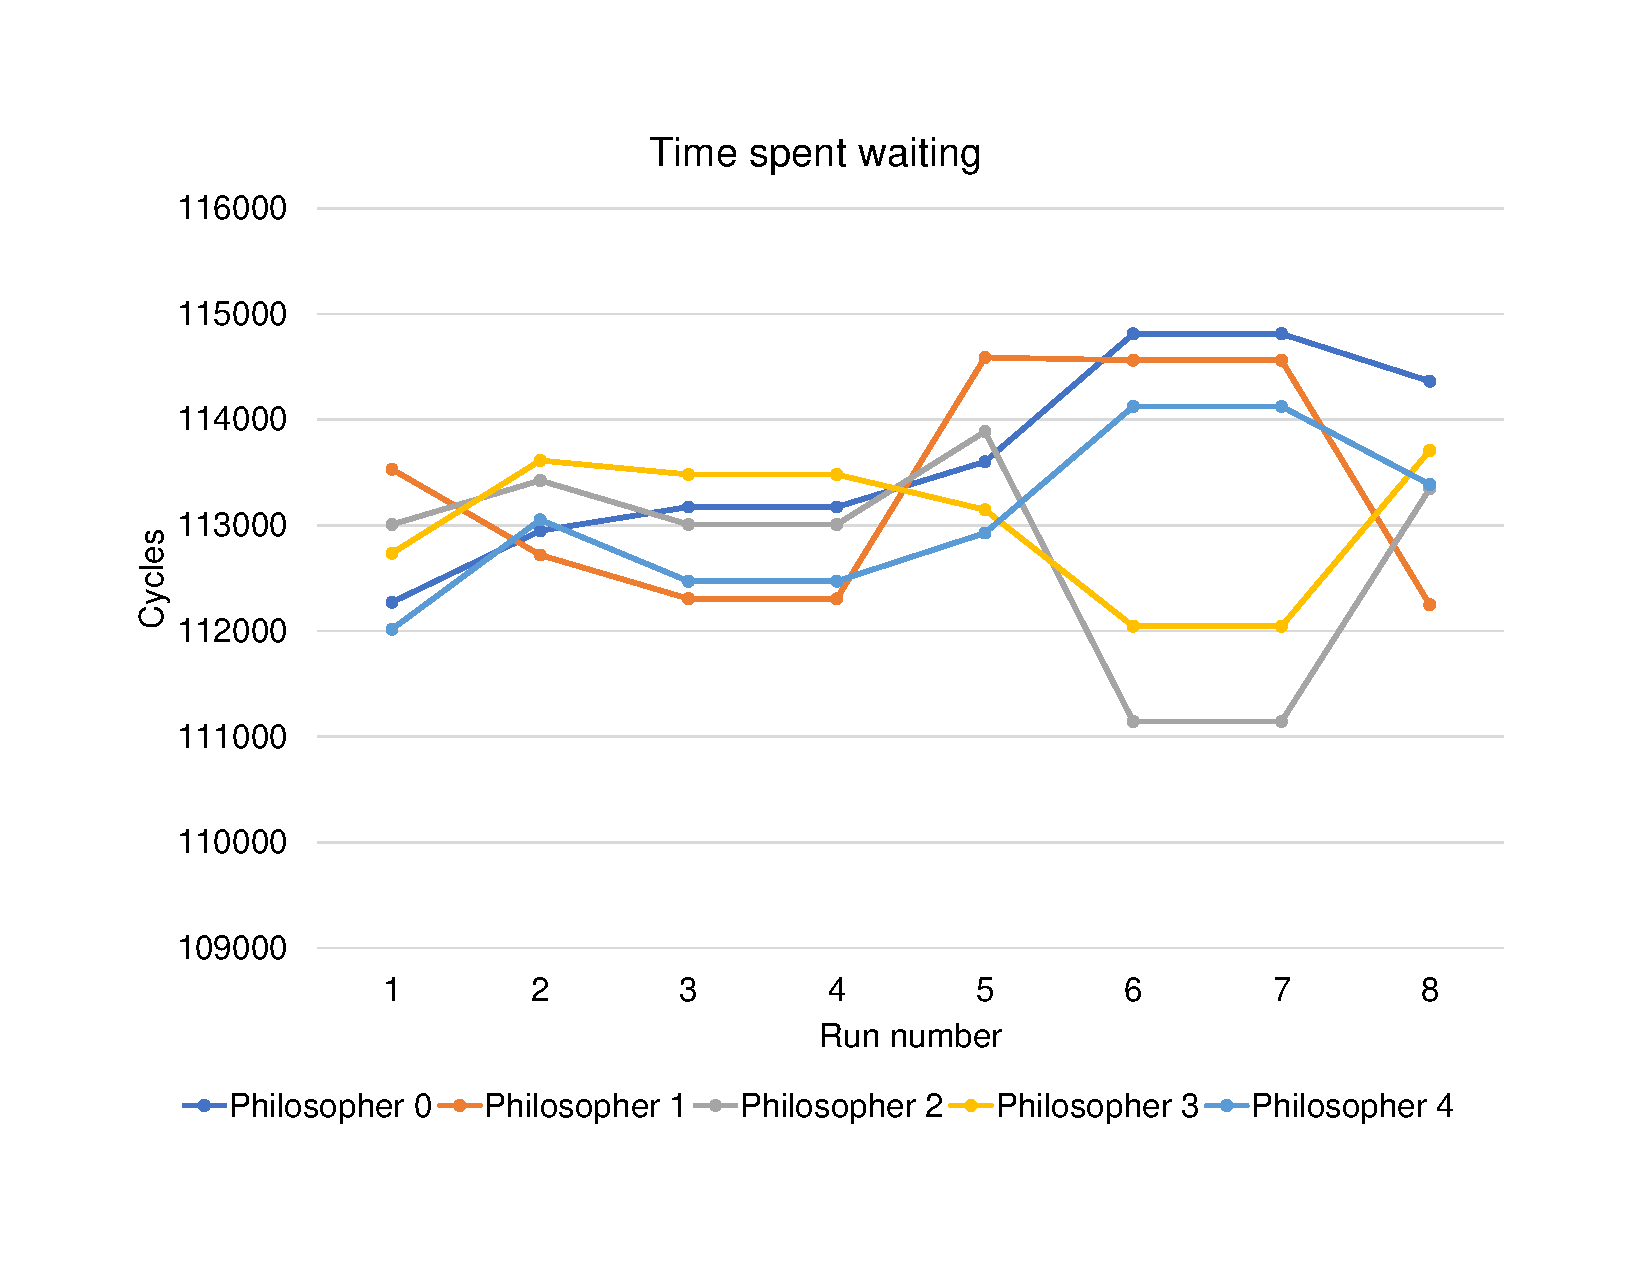
\includegraphics[width=\textwidth]{./resources/waiting-chart.pdf}
    \caption{\sffamily Line chart showing the number of cycles for
      which a philosopher was hungry during simulation across 7
      runs.\\\\}
    \label{fig:waiting-chart} 
  \end{subfigure}
  ~
  \begin{subfigure}[b]{0.3\textwidth}
    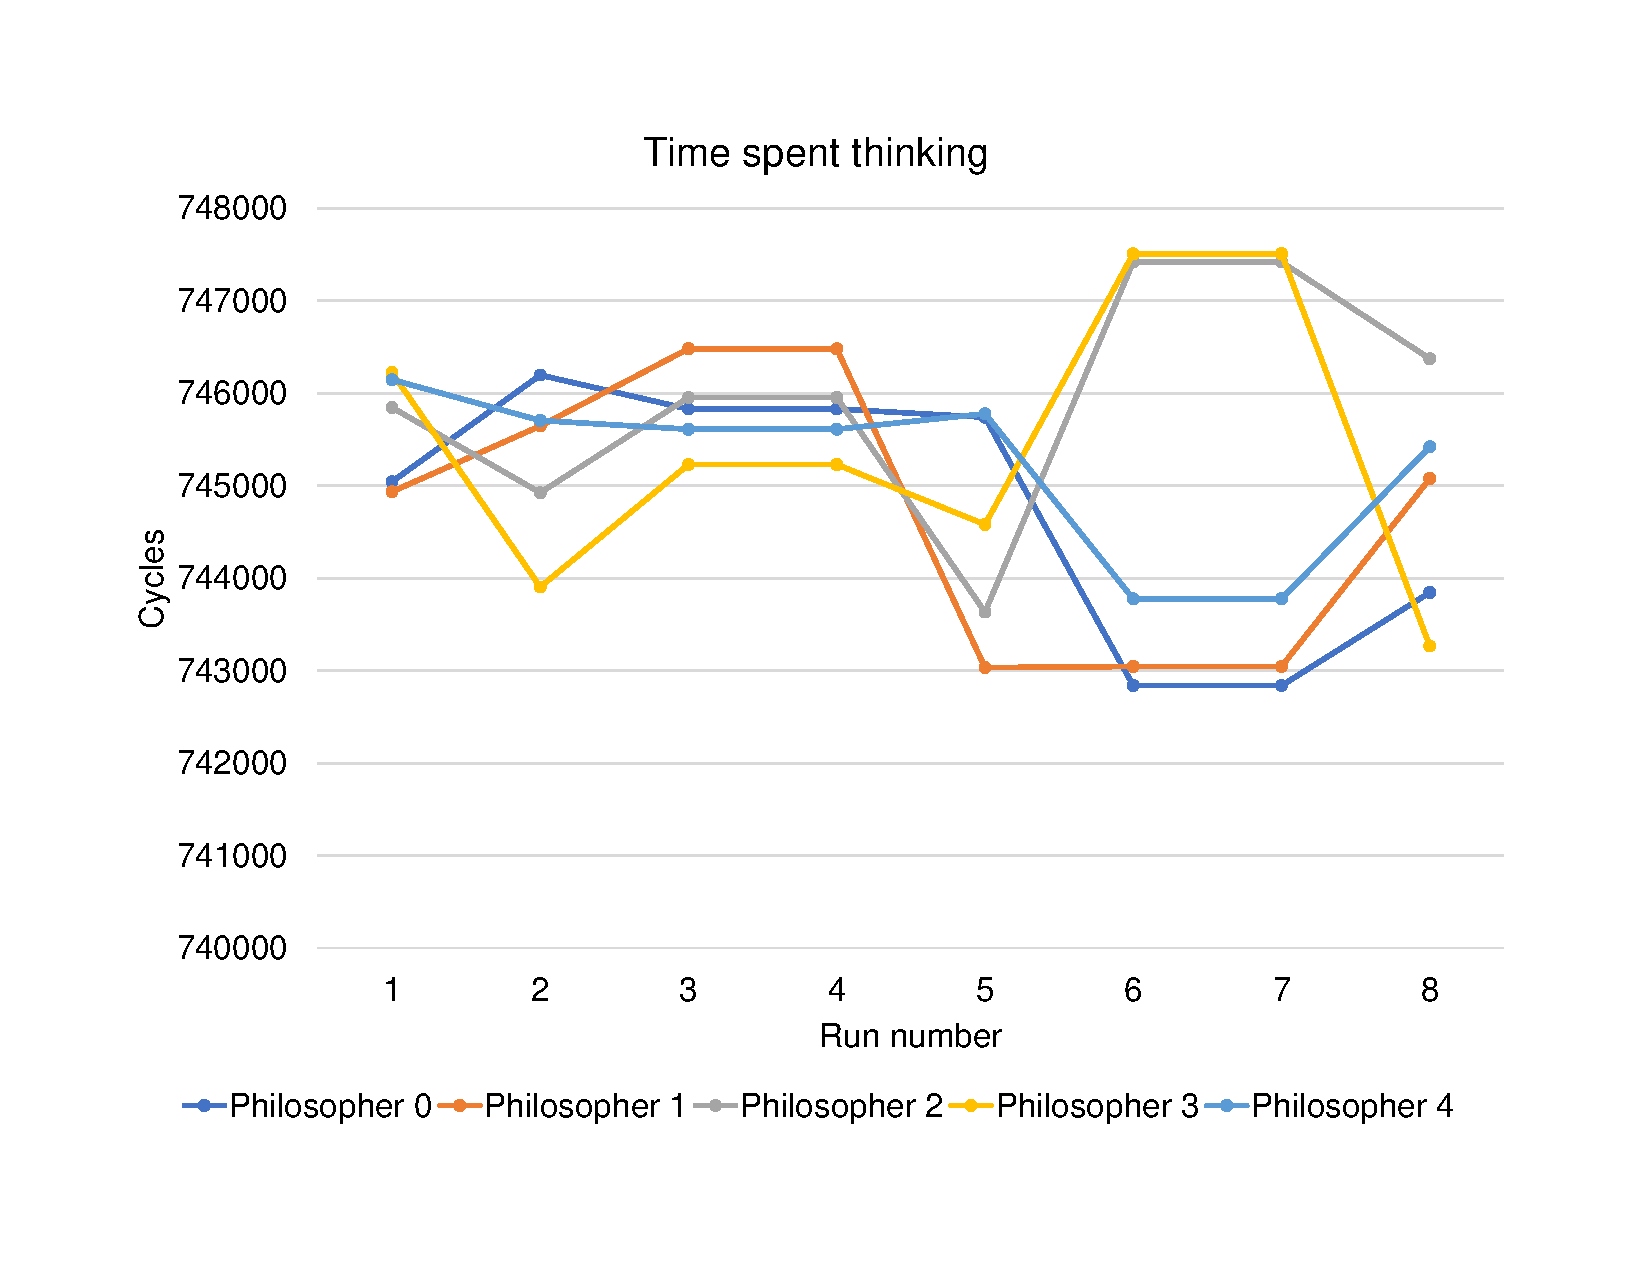
\includegraphics[width=\textwidth]{./resources/thinking-chart.pdf}
    \caption{\sffamily Line chart showing the number of cycles for
      which a philosopher was hungry (that is waiting for atleast of
      the two adjacent chopsticks to be free) during simulation across
      7 runs.}
    \label{fig:thinking-chart}
  \end{subfigure}
  ~
  \begin{subfigure}[b]{0.3\textwidth}
    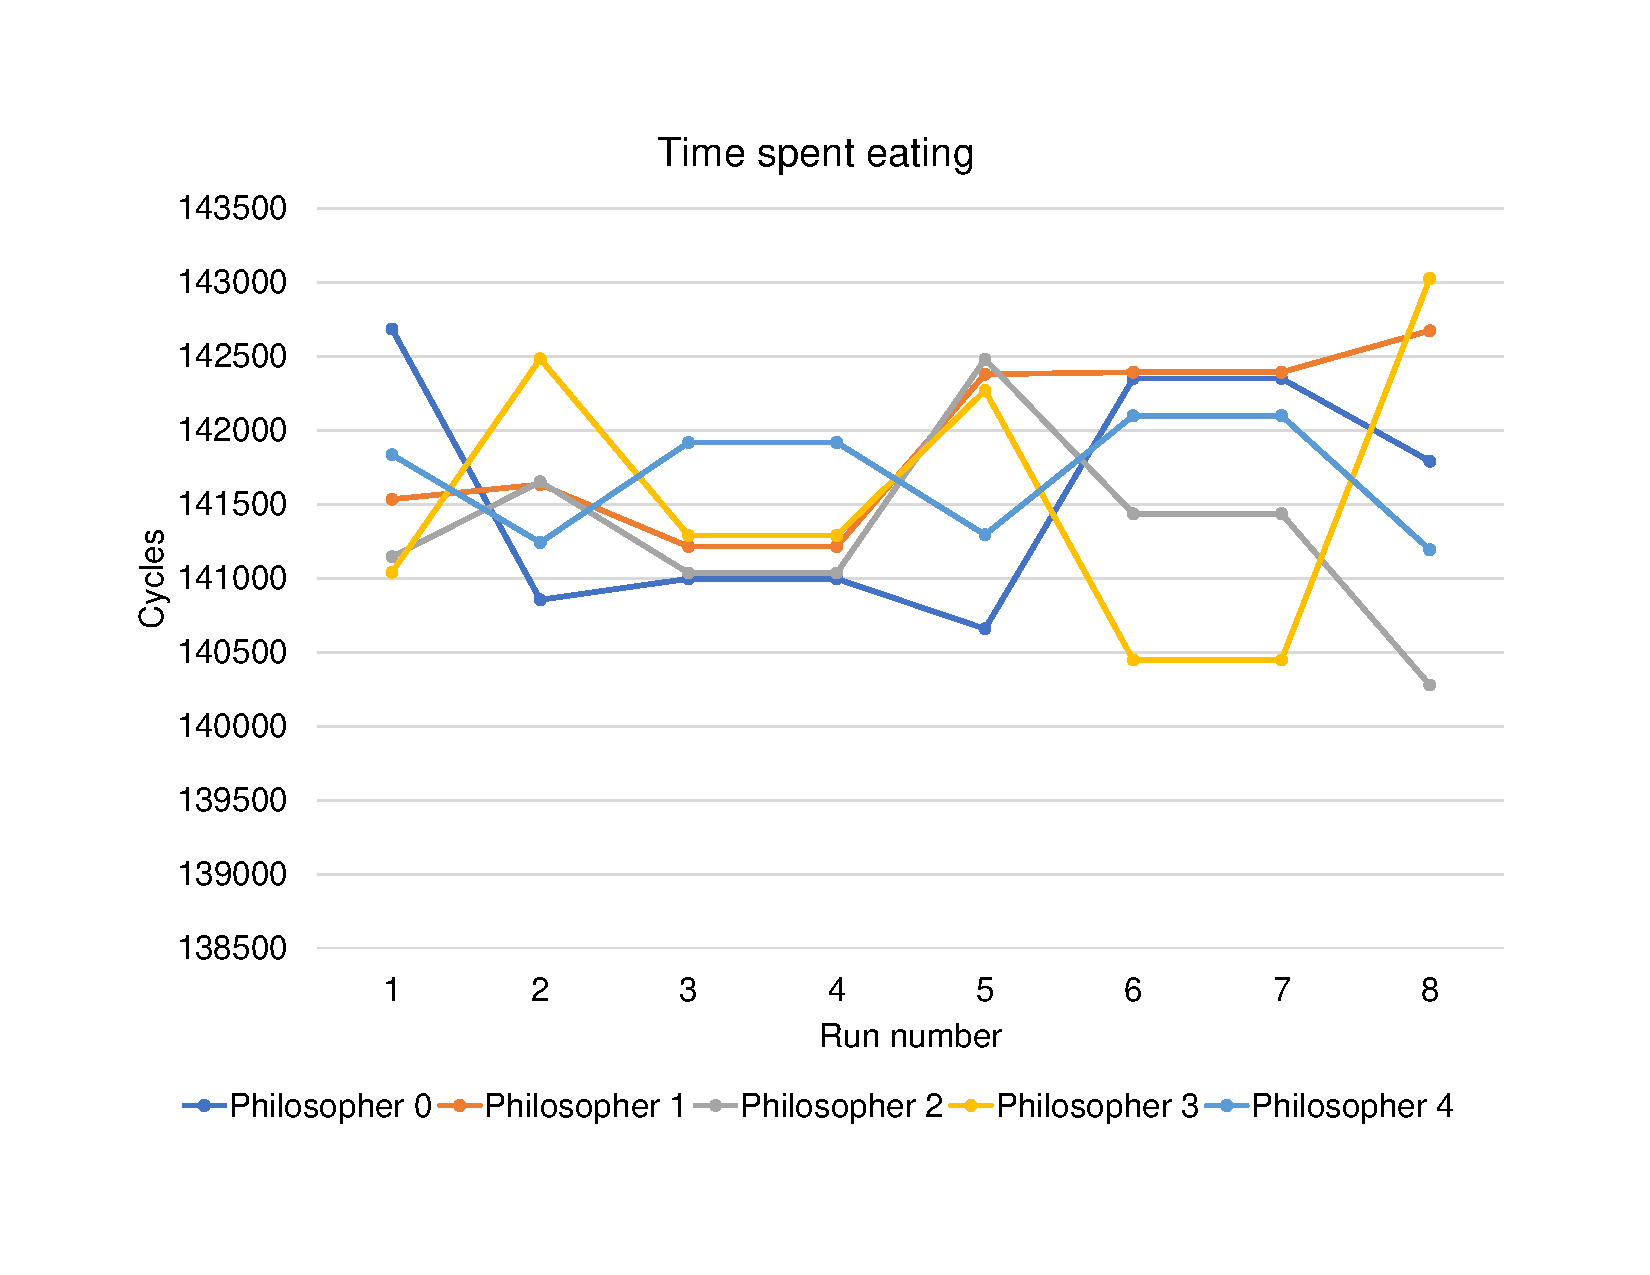
\includegraphics[width=\textwidth]{./resources/time-eating.pdf}
    \caption{\sffamily Line chart showing the number of cycles for
      which a philosopher was eating during simulation across 7
      runs.\\\\}
    \label{fig:time-eating}
  \end{subfigure}
\end{figure}


The problem was written in C and simulated by progressing in steps
(called ticks), total 7 simulations were performed where each one of
them was simulated for 1000000 time quantums (cycles). 5 philosophers
were simulated where each philosopher had a probability of getting
hungry while thinking of 0.05 and probability of going back to
thinking from eating of 0.75 at each cycle. The philosophers had 3
states:

\begin{enumerate}
\item \texttt{HUNGRY}: When a philosopher is waiting for chopsticks.
\item \texttt{EATING}: When a philosopher has acquired two chopsticks
  and is eating.
\item \texttt{THINKING}: When a philosopher is thinking.
\end{enumerate}

\begin{enumerate}
\item[\textbf{\large\sffamily\color{blue}
    Result:}]{\large\sffamily\color{blue} The results clearly show
    that none of the philosophers are at an advantage compared to the
    other and no condition of deadlock arises.}
\end{enumerate}

\section{Code}
\begin{minted}{c}
#include <stdio.h>
#include <math.h>
#include <stdlib.h>
#include <time.h>

const int MAX_TICKS = 1000000;
const int PHILOSOPHER_COUNT = 5;
const int HUNGER_PROBABILITY_MAX = 100;
const int HUNGER_PROBABILITY = 5; /* Out of HUNGER_PROBABILITY_MAX */
const int EATING_PROBABILITY_MAX = 100;
const int EATING_PROBABILITY = 75; /* Out of EATING_PROBABILITY_MAX */

/* Represents the state of a philosopher */
typedef enum phil_state {
    EATING,
    THINKING,
    HUNGRY,
    MAX_PS
} phil_state_t;

/* Represents the state of a chopstick */
typedef enum cs_state {
    BUSY,
    AVAILABLE,
    MAX_CS
} cs_state_t;

/* Represents a philosopher and associated variables */
typedef struct philosopher {
    int id;
    phil_state_t lastState = THINKING;
    phil_state_t state = THINKING;
} philosopher_t;

/* Represents a chopstick and associated variables */
typedef struct chopstick {
    int id;
    cs_state_t state = AVAILABLE;
} chopstick_t;

/* Represents the table on which the philosophers dine together */
typedef struct table {
    philosopher_t *philosophers;
    chopstick_t *chopsticks;
} table_t;

/* Holds statistics of philosopher's different states as an array */
typedef struct stat {
    long int type[MAX_PS];
} stat_t;

/******************************************************************/
/*     Functions for randomly iterating over the philosophers     */
int l_max, l_index, l_offset;
void l_init(int start, int max) {
    l_max = max;
    l_index = start;
    l_offset = rand()%l_max;
}

int l_getCurrentValue() {
    return ((long) l_index * 3 + l_offset) % (l_max);
}

int l_hasNext() {
    return l_index < l_max;
}

int l_next() {
    int answer = l_getCurrentValue();
    l_index++;
    return answer;
}
/******************************************************************/

/* Each call to this function will increase the time by a single tick
 * The function also manages all the philosophers */
long int ticks;
long int tick(table_t *table, long int &ticks, stat_t *philosopherStats) {
    
    ticks++;
    for (int phil = 0; phil < PHILOSOPHER_COUNT; phil++) {	
	/* Philosophers are hungry if the generated random number is
	   greater than HUNGER_PROBABILITY */
	if (table->philosophers[phil].state == THINKING) {
	    phil_state_t newState = (rand()%HUNGER_PROBABILITY_MAX > HUNGER_PROBABILITY)
		? THINKING : HUNGRY;
	    table->philosophers[phil].state = newState;
	} else if (table->philosophers[phil].state == EATING) {
	    phil_state_t newState = (rand()%EATING_PROBABILITY_MAX > EATING_PROBABILITY)
		? THINKING : EATING;
	    if (newState == THINKING) {
		table->philosophers[phil].state = newState;
		
		int right_cs = phil;
		int left_cs = (phil+PHILOSOPHER_COUNT-1)%PHILOSOPHER_COUNT;
		table->chopsticks[left_cs].state  = AVAILABLE;
		table->chopsticks[right_cs].state = AVAILABLE;
	    }
	}
    }

    /* Manage the philosophers */
    l_init(0, PHILOSOPHER_COUNT);
    int phil = 0;
    do {
	phil=l_next();
	printf("phil: %d", phil);
	/* Update the stats */
	philosopherStats[phil].type[table->philosophers[phil].state]++;
	
	if (table->philosophers[phil].state == HUNGRY) {
	    int right_phil = phil+1;
	    int left_phil = (phil+PHILOSOPHER_COUNT-1)%PHILOSOPHER_COUNT;
	    
	    int right_cs = phil;
	    int left_cs = (phil+PHILOSOPHER_COUNT-1)%PHILOSOPHER_COUNT;
	    
	    /* Check if the philosopher's chopsticks are available */
	    if ((table->chopsticks[left_cs].state == AVAILABLE)
		&& (table->chopsticks[right_cs].state == AVAILABLE)) {

		/* If the philosopher's neighbours aren't waiting
		   let's change the state to EATING */
		table->philosophers[phil].state = EATING;
		    
		table->chopsticks[left_cs].state  = BUSY;
		table->chopsticks[right_cs].state = BUSY;
	    }
	}
    } while (l_hasNext());
}

/* Prints the representation of the table passed */
void print_table(table_t *table, int philosopher_count = PHILOSOPHER_COUNT) {
    for (int i = 0; i < PHILOSOPHER_COUNT; i++) {
	switch (table->philosophers[i].state) {
	case THINKING:{
	    printf("T");
	    break;
	}
	case HUNGRY: {
	    printf("H");
	    break;
	}
	case EATING: {
	    printf("E");
	    break;
	}
	}
	printf("%c", table->chopsticks[i].state == BUSY ? '.' : '|');
    }
    printf("\n");
}

/* A function for logging to stdout */
void update_trace(table_t *table, long int &ticks) {
    printf("%04ld: ", ticks);
    print_table(table);
}

/* Prints the stats to the stdout in form of a table */
void print_stats(stat_t *stats) {
    printf("%4s: %6s %6s %6s\n", "id", "eat", "think", "hungry");
    for (int phil = 0; phil < PHILOSOPHER_COUNT; phil++) {
         printf("%4d: %6ld %6ld %6ld\n",
                phil,
                stats[phil].type[0],
                stats[phil].type[1],
                stats[phil].type[2]);
    }
}

/* Main function */
int main() {
    srand(time(NULL));

    stat_t *philosopherStats;
    philosopherStats = (stat*)malloc(sizeof(stat_t)*PHILOSOPHER_COUNT);
	
    /* Initialize the table */
    table_t *table = (table_t*)malloc(sizeof(table_t));
    
    table->philosophers = (philosopher_t*)malloc(sizeof(philosopher_t)*PHILOSOPHER_COUNT);
    for (int phil = 0; phil < PHILOSOPHER_COUNT; phil++) {
	table->philosophers[phil].id = phil;
	table->philosophers[phil].state = THINKING;
    }
    
    table->chopsticks = (chopstick_t*)malloc(sizeof(chopstick_t)*PHILOSOPHER_COUNT);
    for (int cs = 0; cs < PHILOSOPHER_COUNT; cs++) {
	table->chopsticks[cs].id = cs;
	table->chopsticks[cs].state = AVAILABLE;
    }
    printf("Starting simulation...\n");

    int count = 0;
    while (count++ < MAX_TICKS) {
	update_trace(table, ticks);
	tick(table, ticks, philosopherStats);
    }
    printf("\nStats...\n");
    print_stats(philosopherStats);
}

\end{minted}

\subsection{Sample Execution Result}
\begin{verbatim}

 Starting simulation...
 0000: T|T|T|T|T|
 0001: T|T|T|T|T|
 0002: T|T|T|T|T|
 0003: T|T|T|T|T|
 0004: T|T|T|T.E.
 0005: T|T|T|T.E.
 0006: T|T|T|T|T|
 0007: E.T.E.T|T.
 0008: E.T.E.T|T.
 0009: E.T.E.T|T.
 
 Stats...
   id:    eat  think hungry
    0:      2      7      1
    1:      0     10      0
    2:      3      6      1
    3:      0     10      0
    4:      1      8      1

\end{verbatim}
\end{document}
